\documentclass[12pt]{article}

\usepackage{tikz} % картинки в tikz
\usepackage{microtype} % свешивание пунктуации

\usepackage{array} % для столбцов фиксированной ширины



\usepackage{indentfirst} % отступ в первом параграфе

\usepackage{sectsty} % для центрирования названий частей
\allsectionsfont{\centering}

\usepackage{amsmath, amssymb, amsthm} % куча стандартных математических плюшек
\usepackage{amsfonts}
\usepackage{halloweenmath}

\usepackage{graphicx}

%\usepackage{minipage}
\usepackage{tcolorbox}

\usepackage{comment}

\usepackage[top=2cm, left=1.2cm, right=1.2cm, bottom=2cm]{geometry} % размер текста на странице

\usepackage{lastpage} % чтобы узнать номер последней страницы

\usepackage{enumitem} % дополнительные плюшки для списков
%  например \begin{enumerate}[resume] позволяет продолжить нумерацию в новом списке
% \usepackage{caption}

\usepackage{physics}

\usepackage{hyperref} % гиперссылки

\usepackage{multicol} % текст в несколько столбцов

\usepackage{url}

\usepackage{fancyhdr} % весёлые колонтитулы


\usepackage{todonotes} % для вставки в документ заметок о том, что осталось сделать
% \todo{Здесь надо коэффициенты исправить}
% \missingfigure{Здесь будет Последний день Помпеи}
% \listoftodos - печатает все поставленные \todo'шки

% более красивые таблицы
\usepackage{booktabs}
% заповеди из документации:
% 1. Не используйте вертикальные линни
% 2. Не используйте двойные линии
% 3. Единицы измерения - в шапку таблицы
% 4. Не сокращайте .1 вместо 0.1
% 5. Повторяющееся значение повторяйте, а не говорите "то же"

\usepackage{fontspec}
\usepackage{polyglossia}

\setmainlanguage{english}
\setotherlanguages{russian}

% download "Linux Libertine" fonts:
% http://www.linuxlibertine.org/index.php?id=91&L=1
\setmainfont{Linux Libertine O} % or Helvetica, Arial, Cambria
% why do we need \newfontfamily:
% http://tex.stackexchange.com/questions/91507/
\newfontfamily{\cyrillicfonttt}{Linux Libertine O}

\AddEnumerateCounter{\asbuk}{\russian@alph}{щ} % для списков с русскими буквами
\setlist[enumerate, 2]{label=\asbuk*),ref=\asbuk*}

\let\P\relax
\DeclareMathOperator{\P}{\mathbb{P}}
\DeclareMathOperator{\plim}{plim}
\DeclareMathOperator{\E}{\mathbb{E}}
\newcommand{\cN}{\mathcal{N}}
\DeclareMathOperator{\Var}{\mathbb{V}ar}
\DeclareMathOperator{\Cov}{\mathbb{C}ov}
\DeclareMathOperator{\Corr}{\mathbb{C}orr}


\usepackage{epigraph}
\setlength\epigraphwidth{.6\textwidth}
\setlength\epigraphrule{0pt}

\title{День всех влюблённых в тервер}
\date{}

\begin{document}

	\maketitle

\begin{comment}
\section*{Правила}

\newpage

\section*{Наброски идей}
\begin{itemize}
    \item парные состязания: когда один из участников команды вызывает любого противника из другой команды  для решения задачи (в стиле speed dating)
    \item можно свайпать формулы влево с ошибками вправо без (или рисовать на них зелёным и красным)
    \item можно обыграть формат соревнований бодибилдеров: играют два человека, каждый по очереди называет формулу и надо ее обоим написать (правильно). Как хорошо ты знаешь партнера или типа того
\end{itemize}



\section*{Реквизит}

\begin{itemize}
    \item шары, сердечки
    \item очки
    \item гирлянды и свечи 
    \item романтичная музыка
    \item книги
    \item лепестки роз
    \item пицца, пироги, напитки
\end{itemize}

\end{comment}

% \newpage
\section{Задачи для speed dating}
% \newpage

\begin{enumerate}

\item Сваха Зинаида готова искать невесту для любого желающего на $\mathbb{P}$(inder) в течение 60 минут (невеста может быть только одна, поток кандидаток равномерен и они не зависят друг от друга). Вероятность нахождения невесты за указанный период равна 0.1. Если Зинаида не смогла найти подходящую невесту в течение первых 50 минут, какова вероятность того, что за последние 10 минут желающий всё же получит невесту?

Решение: 
A -- невесту нашли на последних 10 минутах,
B -- невесту не нашли на первых 50 минутах
\[ 
\P(A|B) = \frac{\P(A \cap B)}{\P(B)} = \frac{\P(A)}{\P(B)} = \frac{0.1 * 1/6}{ (1 - 0.1) + 0.1 * 1/6} = 0,018
\]

\item На 14 февраля Ванечка раздавал всем девочкам  готовые валентинки, чтобы максимизировать свои шансы на успех. Каждой девочке Ванечка отдал по 3 валентинки, не учитывая их цвет. Валентинки были двух цветов: розовые и красные.  В итоге у 17 девочек оказалось не меньше двух красных валентинок, у 16 девочек не меньше двух розовых валентинок, у 13 точно попалась одна красная и одна розовая валентинка. У скольких девочек все три валентинки были одного цвета? 

Решение: 17 + 16 - 13 = 20

\item Каждый ученик группы после занятий точно ходит или в клуб любителей тервера, или  в клуб любителей финансов, или в клуб любителей микры, или в несколько клубов сразу. В клуб любителей тервера из группы ходят 15 человек, в клуб любителей финансов из группы ходят 7 человек, в клуб любителей микры ходят 22 человека из группы. Совмещают тервер и микру 12 человек, совмещают тервер и финансы 3 человека, совмещают микру и финансы 3 человека. Самая сильная парочка студентов ходит во все 3 клуба. Сколько всего людей в группе?

Решение: 15 + 7 + 22 - 12 - 3 - 3 + 2 = 28

\item В вашей группе 30 человек. 
Сколькими способами можно выбрать из вашей группы четырех человек, чтобы объединить их в команду для Дня влюбленных в тервер? 

 Решение: 29 * 28 * 27 * 26 = 570024 

\item На Вики-страничке по терверу у Елены и Николая 2024 подписчика. 
Ровно половина подписчиков смотрит и очень любит лекции Елены. 
Ровно половина подписчиков смотрит и очень любит семинары Николая. 
При этом оказалось, что ровно 14 подписчиков смотрят и очень любят и лекции, и семинары. Сколько подписчиков ничего не любят?

Решение: 14


\item Предположим, что 5 мужчин из 100 и 25 женщин из 1000 не способны понять и полюбить теорию вероятностей. 
Наугад выбранное лицо не знает формулу вероятности для распределения Пуассона и не видит красоту закона больших чисел и центральной предельной теоремы. Какова вероятность того, что это мужчина?

Решение: 
\[ 
\P ( \text{мужчина}|\text{не любит тервер} ) = \frac{ \P ( \text{мужчина} \cap \text{не любит тервер} ) }{ \P ( \text{не любит тервер} ) } = \frac{ \frac{5}{100} \cdot \frac{1}{2} }{ \frac{5}{100} \cdot \frac{1}{2} + \frac{25}{1000} \cdot \frac{1}{2} } = \frac{2}{3} 
\]

\item Время влюбиться в участника из вашей команды Праздника Влюбленных В Тервер распределено по экспоненциальному закону с параметром равным 0,1. 

Какова вероятность не влюбиться в течение следующих получаса, если прошло уже 15 минут с начала праздника, а Вы еще не влюбились?

Решение:

\[ \P ( \text{ X > 45}|\text{ X > 15} ) = \frac{ \P ( \text{X > 45} \ ) }{ \P ( \text{X > 15} ) } = \frac{ exp ^ { - 0.1 * 45} }{ exp ^ { - 0.1 * 15 } } = \ exp ^ { -3} \]

\item Время, за которое Вы успеете наесться пиццей на Празднике Влюбленных В Тервер распределено по экспоненциальному закону с параметром равным 0.02. 
За сколько минут в среднем Вы наедитесь пиццей? 

Решение:
\[ E(x) = \frac{ 1 }{ 0,02 } = 50 \text{ минут} \] 

\item В вашей команде на Празднике Влюбленных В Тервер помимо вас участвуют два Иннокентия, два Ипполита, Кассандра и Кассиопея. 
Все вместе Вы сели за круглый стол произвольно. 
Какова вероятность, что Вы окажетесь между двумя тёзками? 

Решение:

Слева может сидеть Ипполит1, справа Ипполит2. Или слева Ипполит2, справа Ипполит1. Аналогично с Иннокентиями. Итого нам подходят 4 варианта рассадки тезок, и 4! рассадки всех остальных. Вероятность = $ \frac{ 4 * 4! }{ 6! } $


\item Земфира и Земфир договорились о свидании. 
Земфира обычно не опаздывает на такие встречи, время её опоздания распределено нормально с нулевым средним и ст. отклонением 3 минуты. 
Земфир каждый день решает задачи по терверу и  немного увлекается, поэтому время его опоздания распределено нормально, но с со средним 10 минут и ст. отклонением 10 минут. 
Так как Земфира и Земфир могут переписываться, время опозданий имеет корреляцию 0.2. 

Найдите вероятность того, что их суммарное время опоздания не больше нуля. % (если значение табличное, выпишите для него формулу).

Решение:

$\E(X+Y) = 0 + 10 = 10$

$\Var(X+Y) = \Var(X) + \Var(Y) + 2 \Cov(X, Y) = 9 + 100 + 2 \cdot 3 \cdot 10 \cdot 0.2 = 121$

$\P(X+Y \leq 0) = \Phi(\frac{0-10}{\sqrt{121}}) = \Phi(-10/11) \approx 0.18$


\item Студентка Анфиса готовится к завтрашнему свиданию со своим крашем.
Она знает, что с вероятностью равной 0.5 в Москве будет сильный мороз и снегопад. 
В таком случае ей придется надеть подштанники. 
Однако, ее краш написал ей эсэмэску о том, что завтра будет хорошая погода, поэтому она поменяла свое мнение. 

Посчитайте, с какой вероятностью Анфиса наденет подштанники на свидание, если, с ее точки зрения, краш говорит правду в 70\%  ситуаций.

Решение:

\item  Длина speed datingа для Амфилохия -- случайная величина с функцией плотности 

\begin{equation*}
f_T(t) = 
 \begin{cases}
   IQ \cdot t^2 &\text{если $0 < t < 0.3$ часа}\\
   0 &\text{ иначе. }
 \end{cases}
\end{equation*}

Найдите IQ Амфилохия.

Решение:

$\int_0^{0.3} IQ \cdot t^2  dt = IQ \cdot \frac{0.3^3}{3} = 1, $
$IQ = 111.(1)$

\item 
Лучшие моменты в жизни — проведенные с близкими тебе людьми… (с) Джейсон Стейтем. 
Жизнь Стейтема — непрерывная случайная величина с функцией плотности
\[
f_X(x) = 
 \begin{cases}
   x + \frac{1}{2} &\text{если $0 < x < 1$ }\\
   0 &\text{ иначе. }
 \end{cases}
\]

Найдите второй лучший момент в жизни Стейтема.

Решение:
$\E(X^2) = \int_0^1 x^2 (x + \frac{1}{2}) dx = (\frac{1}{4} x^4 + \frac{1}{6} x^3)|_0^1 = \frac{5}{12} \approx 0.42$
\end{enumerate}
% задача ДЛЯ разбитых сердец и для пока еще целых. Для разбитых: %грустное что-то. про спид-вич-гепатит? 

\newpage
\section{Задачи для ужина}
\begin{enumerate}[resume] % resume стоит, чтобы было проще задачу идентифицировать
\item Преподавательница Ульяна Филиппкина оценивает навыки программирования студентов на языке Gadyuka по шкале от 1 до 6, выставляя каждую оценку равновероятно и независимо от других. 
\begin{enumerate}
    \item Рассчитайте вероятность того, что хотя бы один студент из четырех получит максимальную оценку 6.
    \item Рассчитайте вероятность того, что на занятии, во время которого 48 студентов сидят за партами по двое, хотя бы за одной из парт оба студента получат оценку 6.
    \item Кем в прошлой жизни была Ульяна Филиппкина?
\end{enumerate}
Решение:
Первый случай: 
\[ 
\P (\text{хотя бы один получит 6}) = 1 - \left( \frac{5}{6} \right)^4 \approx 0.5177 
\] 

Второй случай:
\[ 
\P(\text{хотя бы один раз два человека получат 6}) = 1 - \left( \frac{35}{36} \right)^{24} \approx 0.4941 
\]

Первый случай более вероятен.

\item Случайные величины $\xi_1$ и $\xi_2$ описывают силу любви Нюши и Черного Ловеласа и наоборот. 
Силы любви $\xi_1$ и $\xi_2$ независимы и имеют экспоненциальное распределение с интенсивностью $\lambda=1$.
Нюша измеряет индекс любви как $N = \max (\xi_1, \xi_2)$, а Черный Ловелас как $L = \xi_1 + 0.5 \cdot \xi_2$. 
Покажите, что функции распределения индексов любви Нюши и Черного Ловеласа идеально совпадают.

\item Предположим, в студенческой группе 10 девочек и 20 мальчиков. 
Пусть вероятность влюбиться в случайного одногруппника равна $0.05$, а влюбиться в преподавателя курса можно с вероятностью $0.1$ (влюбляться в свой пол почти наверное нельзя). 
Студенты влюбляются независимо и неоднократно.

Что больше: вероятность быть влюблённым мальчику или эта же вероятность для девочки, если курс читает лектор-девушка и семинарист-девушка? \textit{Подсказка: $0.95^3<0.9$}.

Решение:

Для мальчика вероятность не влюбиться ни в кого равна $0.95^{10}\cdot 0.9^2$, для девочки — $0.95^{20}$. 

Заметим,
\[
   0.95^{10} < 0.95\cdot 0.9^6 < 0.9^2.
\]
Таким образом, вероятность не влюбиться ни в кого больше у мальчика, значит ответ: у девочки.

\item Анна и Вронский живут на окружности единичного радиуса $\omega=[0, 2\pi)$, где в точке $0$ располагается центр Москвы, а в точке $\pi$ — Петербурга. 
Про их совместную жизнь известно:
\begin{itemize}
    \item Распределение местоположения Вронского $V$ является равномерным на
    \[
        [\frac{5\pi}{6}, \frac{7\pi}{6}]\cup[\frac{5\pi}{3}, 2\pi)\cup [0, \frac{\pi}{3}]
    \]
    \item Распределение местоположения Анны $A$ является равномерным на
    \[
        [\frac{2\pi}{3}, \frac{4\pi}{3}]\cup[\frac{11\pi}{6}, 2\pi)\cup[0, \frac{\pi}{6}],
    \]
    \item Величины $A$ и $V$ независимы, 
    \item Распределение ($A\;|\;V$) — тоже равномерное, но на
    \[
        \left([\frac{2\pi}{3}, \frac{4\pi}{3}]\cap[V-\frac{\pi}{6}, V+\frac{\pi}{6}]\right)\cup[\frac{11\pi}{6}, 2\pi)\cup[0, \frac{\pi}{6}].
    \]
    % TODO: противоречие между независимостью и разницей условное - безусловное
\end{itemize}


Алексей Александрович Каренин хочет понять
%\begin{enumerate}
%  \item 
    с какой вероятностью его жена (Анна) проводит время с Вронским, если последний находится в Петербурге.

    Математически, требуется найти
    \[
        \P\{|A-V|<\frac{\pi}{6}\;|\;V\in[\frac{5\pi}{6}, \frac{7\pi}{6}]\}.
    \]
%   \item Насколько эта вероятность отличается для случая $(A\;|\;V)=A$?
%   \item (\textit{optional}) Вы бы на месте Алексея Александровича заподозрили неладное?
%\end{enumerate}

Решение: 
\begin{enumerate}
   \item Пусть Вронский находится в точке $t\in[\frac{5\pi}{6}, \frac{7\pi}{6}]$. 
   Обозначим искомую вероятность за $p$.
   Тогда
   \[
   p=\frac{\mathbb P\{|A-V|<\frac{\pi}{6}\;\cap\;V\in[\frac{2\pi}{3}, \frac{4\pi}{3}]\}}{\mathbb P\{V\in[\frac{5\pi}{6}, \frac{7\pi}{6}]\}}=:\frac{p_1}{p_2}.
   \]
   Заметим,
   \begin{align*}
       p_1&=\int_{\frac{5\pi}{6}}^{\frac{7\pi}{6}}\mathbb P\{A\in[t-\frac{\pi}{6}, t+\frac{\pi}{6}]\,|\,V=t\} \cdot f_V(t) dt\\
       &=\int_{\frac{5\pi}{6}}^{\frac{7\pi}{6}}\frac{1}{2}\cdot \frac{1}{\pi}dt\\
       &=\frac{1}{2\pi}\left(\frac{7\pi}{6}-\frac{5\pi}{6}\right)\\
       &=\frac{1}{6}.
   \end{align*}
    
   Так как $p_2=\frac{1}{3}$, получаем ответ $\frac{1}{2}$.

   \item В таком случае
   \begin{align*}
       p_1&=\int_{\frac{5\pi}{6}}^{\frac{7\pi}{6}}\mathbb P\{A\in[t-\frac{\pi}{6}, t+\frac{\pi}{6}]\,|\,V=t\} \cdot f_V(t) dt\\
       &=\int_{\frac{5\pi}{6}}^{\frac{7\pi}{6}}\mathbb P\{A\in[t-\frac{\pi}{6}, t+\frac{\pi}{6}]\} \cdot f_V(t) dt\\
       &=\int_{\frac{5\pi}{6}}^{\frac{7\pi}{6}}\frac{1}{3}\cdot \frac{1}{\pi}dt\\
       &=\frac{1}{3\pi}\left(\frac{7\pi}{6}-\frac{5\pi}{6}\right)\\
       &=\frac{1}{9}.
   \end{align*}

   \item Вероятность возрастает с $1/9=0.111$ до $1/6=0.166$. 
   Пять процентных пунктов звучит как не очень большая разница...
\end{enumerate}

\item По сюжету песни «Миллион алых роз» художник расположил у окна героини «целое море цветов» — формализуем это понятие.

Пусть Алла Борисовна живёт в одномерном пространстве в точке $0$. 
Художник раскладывает цветы в луч, каждый цветок описывается полуинтервалом $(a, b]$, где $0\le a< b$. 
Рассмотрим произвольное «море цветов» 
\[
    F=\bigcup_{i=1}^{1000000} \,(a_i, b_i].
\]
Рассмотрим систему «морей цветов»
\[
    \mathcal{F}=\left\{F\;\bigg\rvert\;0<a_i<b_i\le+\infty\;\forall i\right\}\cup\emptyset.
\]

\begin{enumerate}
    \item Как вы мыслите объект «море цветов»? Напишите хокку\footnote{Стихотворение без рифм, в три строчки: в первой 5 слогов, потом 7 и снова 5.}.
    \item Как вы мыслите множество $\mathcal{F}$? 
    Напишите хокку.
    \item Среди поклонников Аллы Борисовны популярна алгебраическая структура «алгебра».
    Система множеств $S$ является алгеброй, если 
    \begin{itemize}
        \item $\emptyset\in S$;
        \item найдётся $\Omega\in S$ такое, что любой элемент $A\in S$ является подмножеством $\Omega$;
        \item $A\in S\Rightarrow A^c:=\Omega\setminus A\in S$;
        \item операция пересечения не выводит за рамки $S$. 
    \end{itemize}
    Является ли $\mathcal{F}$ алгеброй?
    \item Является ли $\mathcal{F}$ $\sigma$-алгеброй?
    (Бывалые поклонники Аллы Борисовны помнят, что для этого операция счётного объединения не должна выводить за рамки $S$.)
    
\end{enumerate}

Решение
\begin{enumerate}
   \item Луч из цветов: | есть место между ними, | или вовсе нет.
  \item Хоть как их клади — | все способы описать | может система.
   \item Пустое лежит в $F$; также $\Omega=(0, +\infty]$; к тому же, дополнение к любому полуотрезку есть объединение двух других полуотрезков; а пересечение — если не пустое — имеет вид того же полуотрезка.
   \item Нет, контрпример — произвольное разбиение $(0, +\infty)$. 
  (Объединение элементов разбиения не представимо как объединение миллиона полуотрезков.)
\end{enumerate}
\item Машенька из города Иваново хочет, чтобы у ее избранника был доход выше среднего и IQ выше среднего. 

В городе Иваново доход мужчин в тысячах рублей, $X$, и IQ мужчин, $Y$,  имеют совместное нормальное\footnote{В Иваново чтут статью 6.21 КоАП РФ и статьи 280-282 Уголовного кодекса.} распределение 
\[
\begin{pmatrix}
    X \\
    Y
\end{pmatrix} \sim \cN \left(
\begin{pmatrix}
    30 \\
    100
\end{pmatrix},
\begin{pmatrix}
    16 & 18 \\
    18 & 81
\end{pmatrix}
\right)
\]

\begin{enumerate}
\item Какова вероятность встретить избранника с подходящим уровнем дохода?
\item Судя по первой встрече в кафе, у Ванечки IQ равен 110. 
Какова условная вероятность того, что Ванечка подходит Машеньке?
% \item Какова вероятность того, что Машеньке подходит случайно встреченный в баре Михаил?
% \item Судя по первой встрече в кафе, у Ванечки IQ выше среднего. 
% \item Какова условная вероятность того, что Ванечка подходит Машеньке?
% \item Как зависит вероятность в пункте (в) от коэффициента корреляции?
\item Какова вероятность того, что \emph{к} Машеньке подойдёт случайно встреченный в баре Михаил?
\end{enumerate}

Решение:
\begin{enumerate}
\item $\P(X > 30) = 1/2$, 2 балла
\item $\P(X > 30 \mid Y = 110)$, 7 баллов
\[
X = 18/81 Y + U
\]
\[
\Var(X) = (18/81)^2 \Var(X) + \Var(Y)
\]
\[
\Var(U) = 12
\]
\[
\E(X \mid Y = 110) = 
\]

%\item $\P(X > 30, Y > 100)$
%\item $\P(X > 30 \mid Y > 100)$
%\item 
\item вопрос шутка, принимаем любой ответ! 1 балл
\end{enumerate}

\

\item Нюша не совсем уверена в своей любви к Барашу, поэтому она решила погадать на цветах, а именно на двух ромашках. 
На каждой ромашке изначально ровно $N$ лепестков. 
Нюша выбирает равновероятно цветок наугад и вырывает один лепесток. 
Затем снова выбирает цветок наугад и снова вырывает один лепесток, и так далее.

Какова вероятность того, что, когда один из цветков окажется пустым, на втором останется ровно $m$ лепестков?

Решение: Если первый цветок оказался пустой, а второй содержит m лепестков, то это означает, что всего было сорвано $2N -m$ лепестков, причем $N$ штук было сорвано с одного цветка и последний лепесток был сорван с того же цветка. Умножаем вероятность на 2, так как ситуация аналогична для двух цветков.
\[ \P ( \text{один цветок пустой} | \text{на другом цветке } m \text{ лепестков}) = 2 \cdot C_{2N-m-1}^{m-1} \cdot \frac{1}{2^{2N-m}} = \frac{1}{2^{2N-m-1}} \cdot C_{2N-m-1}^{m-1} \]


\item Случайная величина \(LoveTime\) — время, которое парень Антон уделяет  на ухаживание за своей девушкой Полиной — имеет ненормальное распределение вида 
\(F(mwah|Mwah>0)\), где \(Mwah\) — нормально распределенная случайная величина с математическим ожиданием, равным двум часам и стандартным отклонением, равным одному часу.

Полина расстанется со своим парнем в день, когда он уделит ей меньше двух часов своего времени. Найдите вероятность того, что Полина и Антон перестанут встречаться. Округлите ответ до трех знаков после запятой.

\item У Вовы было бесконечное количество мәхәббәт пыяласы, которые он бросал. Вероятность того, что мәхәббәт пыяласының ватылган, равна 0.6. Вова кидал мәхәббәт пыяласын до тех пор, пока не ватты два подряд. Найдите ожидаемое количество брошенных мәхәббәт пыяласының (округляя вверх до целого числа).

Решение:
X -- число брошенных пыяласын; 1 -- ватылды; 0 -- ватылмады.

Условно на первый бросок $\E(X) = \E(X|1) \cdot \P(1) + \E(X|0) \cdot \P(0) = \E(X|1) \cdot 0.6 + (1 + \E(X)) \cdot 0.4$

Условно на два броска $\E(X|1) = \E(X|1,1) \cdot 0.6 + \E(X|1,0) \cdot 0.4 = 2 \ \cdot 0.6 + (2 + \E(X)) \cdot 0.4$

В итоге $\E(X) = \frac{1 + 0.6}{0.6 ^ 2} = 4.(4) \approx 5$

\end{enumerate}

\newpage
\section{Задачи для $\P$индера}

Оформляем задания как тиндер-аккаунты с фото.
Имена до буквы с А по M — верные ответы, с N по Z — неверные.
Имена пишем на английском, чтобы ближе к стилистике tinder. 

\begin{enumerate}
\item В связке воздушных шариков $N$ шаров — белые, а $K$ шаров — розовые. 
Вероятность того, что ровно $k$ из $n$ случайно взятых шаров — розовые, равна
\[ 
\P (X = k) = \frac{C_K^k \cdot C_N^{n-k}}{C_{N+K}^n} 
\]

% \item Пусть $X_n$ — последовательность случайных величин. Верно ли, что сходимость по вероятности определяется равенством 


\item Пусть $X$, $Y$ — случайные величины, имеющие совместное нормальность распределение с параметрами $\E(X) = \mu_X$, $\E(Y) = \mu_Y$, $\Var(X) = \sigma_X^2$, $\Var(Y) = \sigma_Y^2$, $\Corr(X, Y) = \rho$. Верно ли, что совместная плотность $X, Y$ имеет следующий вид
\[ 
f_{X, Y} (x, y) = \frac{1}{2\pi \sigma_X \sigma_Y \sqrt{1 - \rho^2} } \exp \left( \frac{1}{1-\rho^2} \left( \frac{(x - \mu_X)^2}{2\sigma_X^2} + \frac{(y - \mu_Y)^2}{2\sigma_Y^2} - \rho \frac{(x - \mu_X)(y - \mu_Y)}{\sigma_X \sigma_Y} \right) \right)    
\]

%аксиоматика и простые вероятности
\item (неверно) Корректной $\Omega$  для эксперимента с подбрасыванием монетки является: 
\[
\Omega = \{\text{Орёл и идёт дождь}, \text{Решка и дождя нет}, \text{Решка}\}
\]

\end{enumerate}

\newpage
\newtcolorbox{tinderm}[1]{colback=blue!5!white,
colframe=blue!75!black,fonttitle=\bfseries,
title={#1}}

\newtcolorbox{tinderf}[1]{colback=pink!5!white,
colframe=pink!90!black,fonttitle=\bfseries,
title={#1}}


\newtcbox{\xbox}[1][black]{on line,
arc=7pt,colback=#1!10!white,colframe=#1!50!black,
before upper={\rule[-3pt]{0pt}{10pt}},boxrule=1pt,
boxsep=0pt,left=6pt,right=6pt,top=2pt,bottom=2pt}

\newtcolorbox{mybox}{colback=yellow!5!white,
colframe=yellow!75!black}


\begin{minipage}{0.45\textwidth}
\begin{tinderm}{Pasha 20}

\includegraphics[width=\textwidth]{tinder-photo/pasha.png}

\xbox[green]{OLS} \xbox{DID} \xbox[blue]{RDD}

\begin{mybox}
Формула условной вероятности:
\[
\P(A \mid B) = \frac{\P(A \cup  B)}{\P(B)}.
\]
\end{mybox}
\end{tinderm}
\end{minipage}
%
%
\begin{minipage}{0.45\textwidth}
\begin{tinderm}{Nikita 21}

\includegraphics[width=\textwidth]{tinder-photo/nikita.png}

\xbox[green]{GMM} \xbox{FED} \xbox[blue]{Bootstrap}

\begin{mybox}
Для любой величины $X$ и любого $\varepsilon>0$:
\[
\P (X \leq \varepsilon) \leq \frac{\E(X)}{\varepsilon}.
\]
\end{mybox}
\end{tinderm}
\end{minipage}

\begin{minipage}{0.45\textwidth}
\begin{tinderf}{Ekaterina 20}
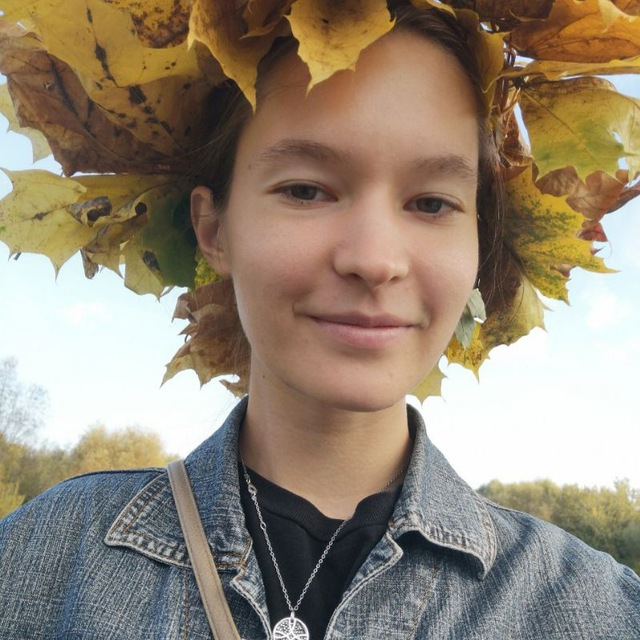
\includegraphics[width=\textwidth]{tinder-photo/ekaterina.jpg}

\xbox[green]{Bayes} \xbox{LLN} \xbox[blue]{MLE}

\begin{mybox}
Во множестве из $n$ элементов ровно $2^n$ подмножеств. 
\end{mybox}
\end{tinderf}
\end{minipage}
%
%
\begin{minipage}{0.45\textwidth}
\begin{tinderf}{Evelina 20}

\includegraphics[width=\textwidth]{tinder-photo/tinder-evelina.jpg}

\xbox[green]{LLN} \xbox{Bayes} \xbox[blue]{MLE}

\begin{mybox}
Корректная $\Omega$  для эксперимента с подбрасыванием монетки:
\[
\Omega = \left\{\begin{array}{l}
\text{Орёл и идёт дождь},\\
\text{Орёл и дождя нет},\\
\text{Решка}
\end{array}\right\}.
\]
\end{mybox}
\end{tinderf}
\end{minipage}

\begin{minipage}{0.45\textwidth}
\begin{tinderm}{Ivan 21}

\includegraphics[width=\textwidth]{tinder-photo/ivan.jpg}

\xbox[green]{GMM} \xbox{ML} \xbox[blue]{CLT}

\begin{mybox}
Для любого $a \in \mathbb{R}$ верно:
\[
\E(\xi -a)^2 \ge \Var(\xi).
\]
\end{mybox}
\end{tinderm}
\end{minipage}
%
%
\begin{minipage}{0.45\textwidth}
\begin{tinderm}{Ulyan 30}
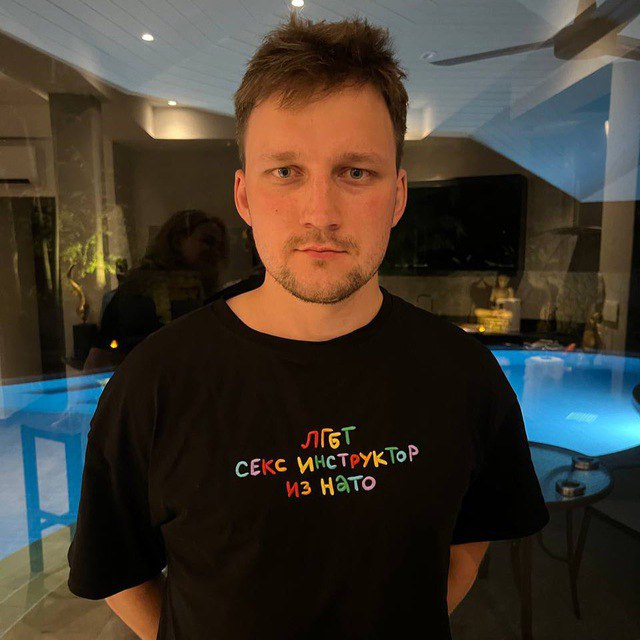
\includegraphics[width=\textwidth]{tinder-photo/filipp.jpg}

\xbox[green]{TF--IDF} \xbox{FitFetish} \xbox[blue]{W2V}

\begin{mybox}
 Если $\E(X \cdot Y) = \E(X) \cdot \E(Y)$, то $X$ и $Y$ — независимы.
\end{mybox}
\end{tinderm}
\end{minipage}

\begin{minipage}{0.45\textwidth}
\begin{tinderm}{Boris 43}
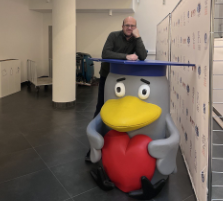
\includegraphics[width=\textwidth]{tinder-photo/boris.png}

\xbox[green]{Bootstrap} \xbox{GitHub} \xbox[blue]{BDSM}

\begin{mybox}
Если $\P(A) = 1$ и $\P(B)=1$, то события $A$ и $B$ независимы.
\end{mybox}
\end{tinderm}
\end{minipage}
%
%
\begin{minipage}{0.45\textwidth}
\begin{tinderm}{Bogdan 20}

\includegraphics[width=\textwidth]{tinder-photo/bogdan.png}

\xbox[green]{Trees} \xbox{Blackboard} \xbox[blue]{Integral Calculus}

\begin{mybox}
\[
\P(A \cap B) \ge \P(A) + \P(B) - 1.
\]
\end{mybox}
\end{tinderm}
\end{minipage}





\begin{minipage}{0.45\textwidth}
\begin{tinderm}{Dmitrii 21}

\includegraphics[width=\textwidth]{tinder-photo/dmitrii.png}
\xbox[green]{SDE} \xbox{LLN} \xbox[blue]{CLT}
\begin{mybox}
Если $S$ — это сумма очков на трёх выпавших кубиках, то:
\[
\P(S = 11) > \P(S = 12).
\]
\end{mybox}
\end{tinderm}
\end{minipage}
%
%
\begin{minipage}{0.45\textwidth}
\begin{tinderm}{Daniil 20}

\includegraphics[width=\textwidth]{tinder-photo/daniil.png}

\xbox[green]{RamseyTest} \xbox{SUR} \xbox[blue]{2SLS}

\begin{mybox}
Существуют $2024$ случайных события, такие, что любые $2023$ из них — независимы, а все они вместе — зависимы.
\end{mybox}
\end{tinderm}
\end{minipage}



\begin{minipage}{0.45\textwidth}
\begin{tinderm}{Andrey 20}

\includegraphics[width=\textwidth]{tinder-photo/andrey_2.png}

\xbox[green]{HatMatrix} \xbox{StochAn} \xbox[blue]{52}

\begin{mybox}
Для любой случайной величины верно:
\[
\E(X^2) \ge \E(X)^2.
\]
\end{mybox}
\end{tinderm}
\end{minipage}
%
%
\begin{minipage}{0.45\textwidth}
\begin{tinderf}{Anna 19}

\includegraphics[width=\textwidth]{tinder-photo/anna.png}

\xbox[green]{Jensen's Inequality} \xbox{CLT} \xbox[blue]{Poisson}

\begin{mybox}
Если $A \subset \Omega$, то события $A$ и $\Omega$ независимы.
\end{mybox}
\end{tinderf}
\end{minipage}
%
\newpage
\begin{minipage}{0.45\textwidth}
\begin{tinderm}{Vsevolod 20}
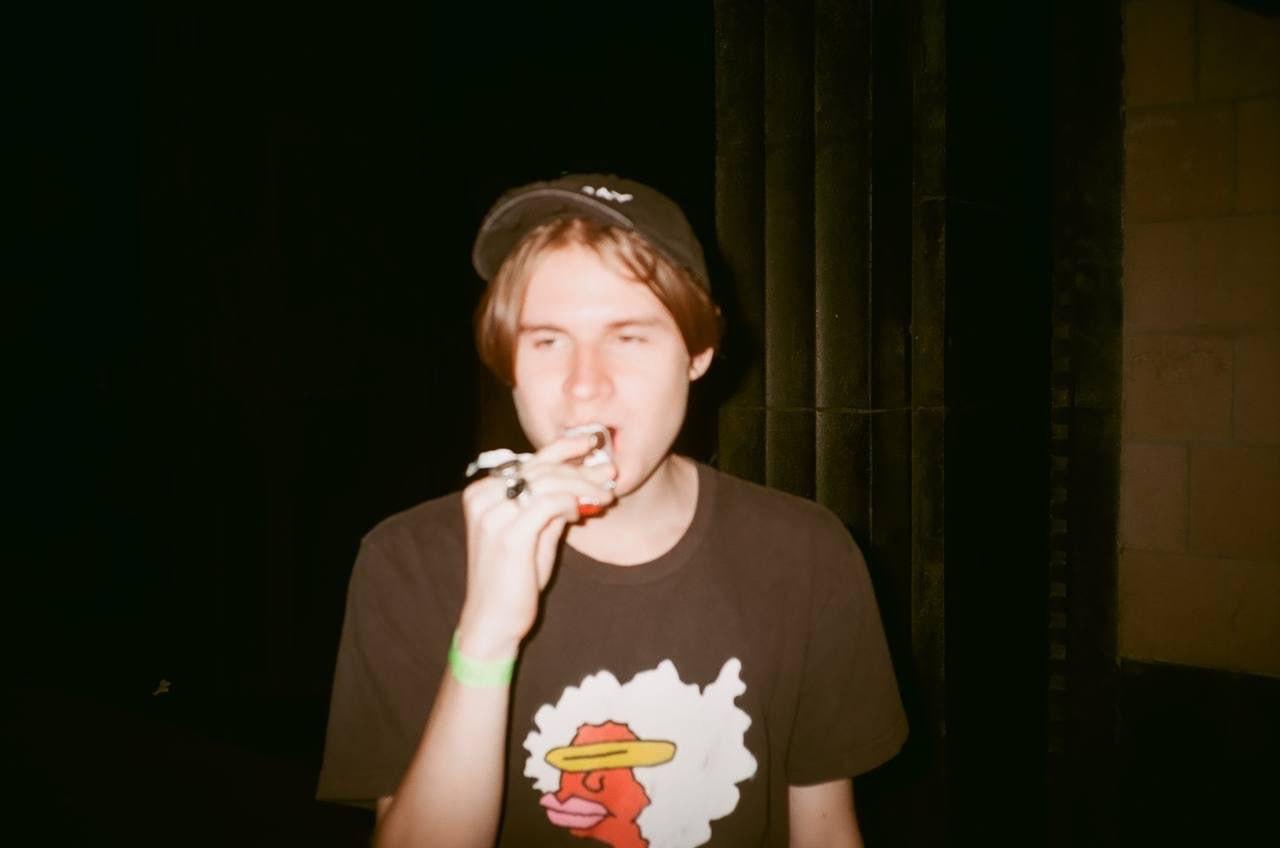
\includegraphics[width=\textwidth]{tinder-photo/paramonov.jpg}

\xbox[green]{SGD} \xbox{LLN} \xbox[blue]{ML}

\begin{mybox}
Для любой величины $X$ и любого $c < 0$: 
\[
\P(|X - \mu| \geq c) \leq \frac{\sigma^2}{c^2}.
\]
\end{mybox}
\end{tinderm}
\end{minipage}
%
%
\begin{minipage}{0.45\textwidth}
\begin{tinderm}{Andrey 20}
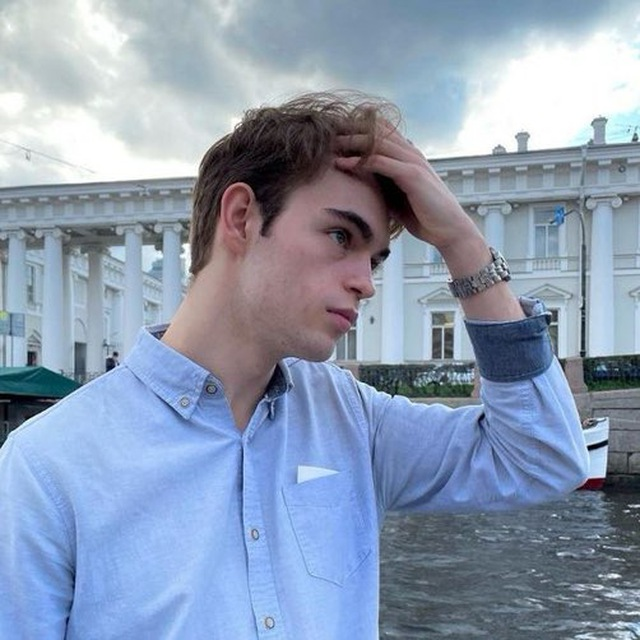
\includegraphics[width=\textwidth]{tinder-photo/andrey.jpg}

\xbox[green]{T513} \xbox{Studsovet} \xbox[blue]{DL}

\begin{mybox}
\[
(A \cup B)^c = A^c \cap B^c.
\]
\end{mybox}
\end{tinderm}
\end{minipage}

\begin{minipage}{0.45\textwidth}
\begin{tinderm}{Richard 20}
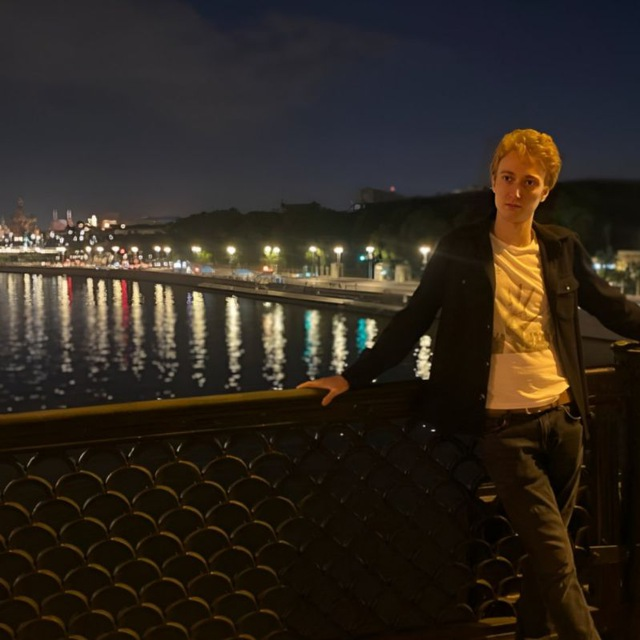
\includegraphics[width=\textwidth]{tinder-photo/richard.jpg}

\xbox[green]{ML} \xbox{GBoost} \xbox[blue]{CATE}

\begin{mybox}
\[
\P(A|B) + \P(A|B^c) = 1.
\]
\end{mybox}
\end{tinderm}
\end{minipage}
%
%
\begin{minipage}{0.45\textwidth}
\begin{tinderf}{Mariya 28}
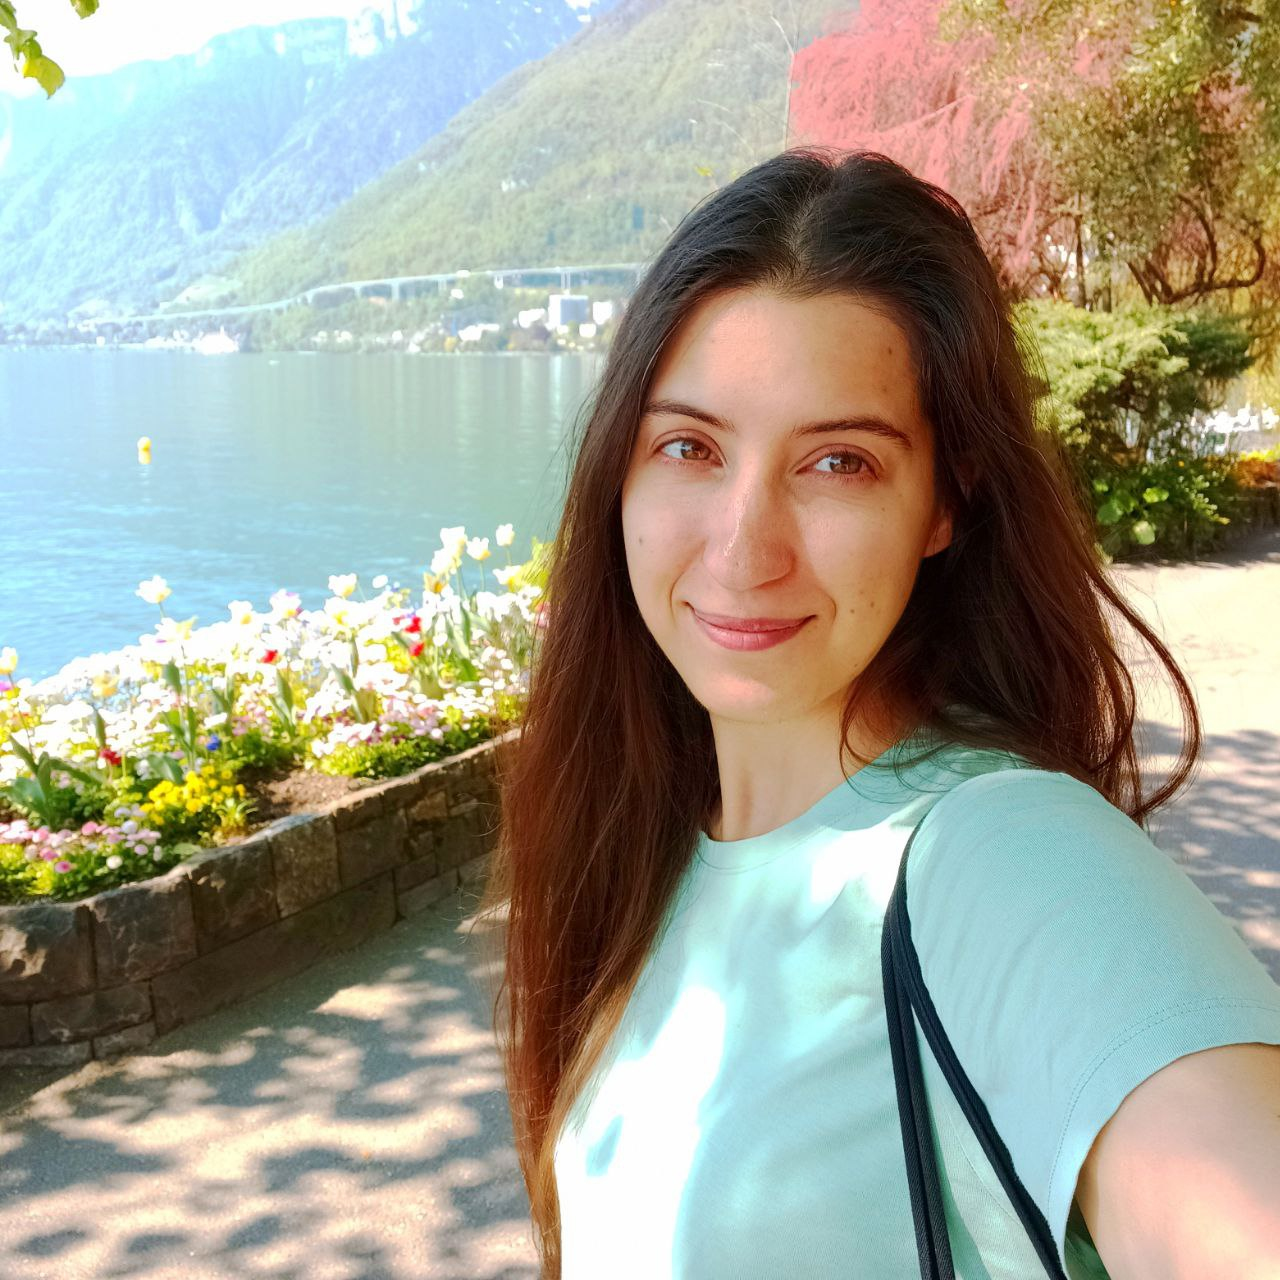
\includegraphics[width=\textwidth]{tinder-photo/mariya.jpg}

\xbox[green]{VAR} \xbox{ETS} \xbox[blue]{Black--Scholes}

\begin{mybox}
Если события  $A$ и $B$ независимы, то события $A^c$ и $B^c$ тоже независимы.
\end{mybox}
\end{tinderf}
\end{minipage}



\begin{minipage}{0.45\textwidth}
\begin{tinderm}{Nikita 19}

\includegraphics[width=\textwidth]{tinder-photo/nikita2.jpg}

\xbox[green]{CLT} \xbox{Bayes} \xbox[blue]{LLN}

\begin{mybox}
Случайные величины $\xi$ и $\arcsin(\xi)$ независимы.
\end{mybox}
\end{tinderm}
\end{minipage}
%
%
\begin{minipage}{0.45\textwidth}
\begin{tinderm}{Vladimir 20}

\includegraphics[width=\textwidth]{tinder-photo/vladimir.jpg}

\xbox[green]{PCA} \xbox{WLS} \xbox[blue]{SEM}
\begin{mybox}
$n$ валентинок можно разложить по порядку $(n-1)!$ способами.
\end{mybox}
\end{tinderm}
\end{minipage}


\begin{minipage}{0.45\textwidth}
\begin{tinderf}{Bella 28}
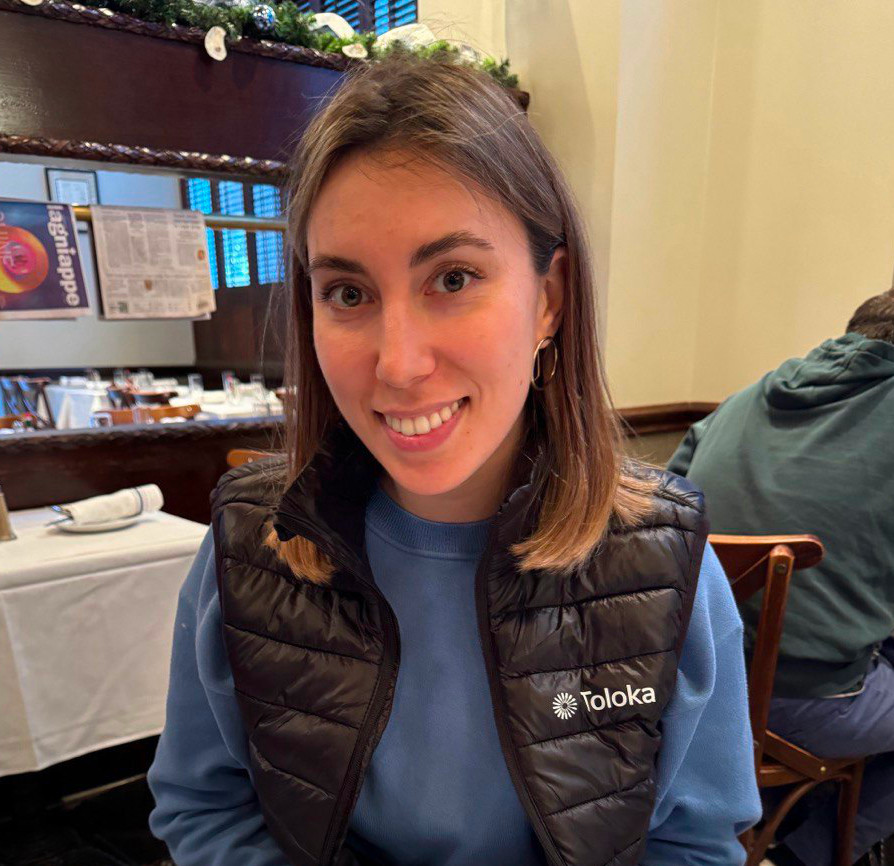
\includegraphics[width=\textwidth]{tinder-photo/bella.jpeg}

\xbox[green]{ProbabilityTheory} \xbox{GitHub} \xbox[blue]{Finance}

\begin{mybox}
Если $N$ — независимая от $X_1$, $X_2$, \ldots{ } случайная величина, то: 
\[
\E(X_1 + \ldots + X_N)= \E(N)\E(X).
\]
\end{mybox}
\end{tinderf}
\end{minipage}
%
%
\begin{minipage}{0.45\textwidth}
\begin{tinderm}{Timur 20}
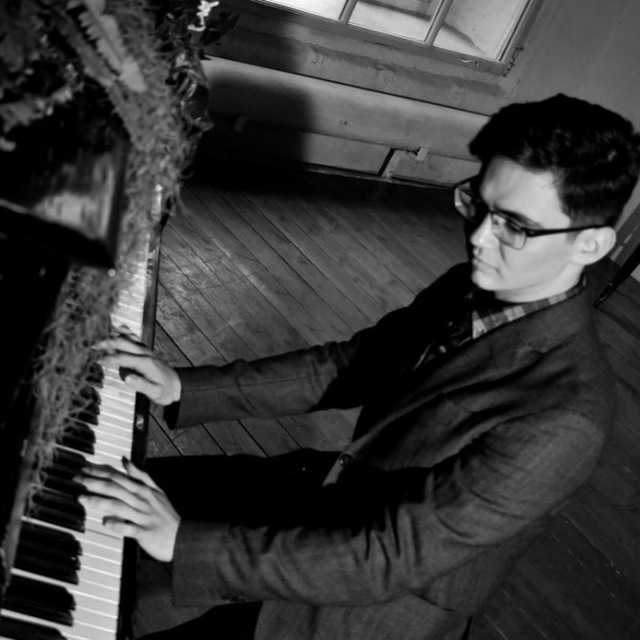
\includegraphics[width=\textwidth]{tinder-photo/timur.jpg}

\xbox[green]{ATET} \xbox{Finance} \xbox[blue]{GARCH}

\begin{mybox}
Существуют такие события $A$ и $B$, что $\P(A \cap B^c) = \P(B \cap A^c) = \frac{4}{7}$.
\end{mybox}
\end{tinderm}
\end{minipage}

\newpage
\begin{minipage}{0.45\textwidth}
\begin{tinderf}{Alyona 21}
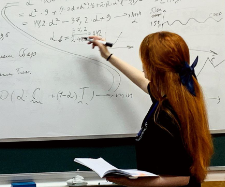
\includegraphics[width=\textwidth]{tinder-photo/alyona.png}

\xbox[green]{DSGE} \xbox{ONS} \xbox[blue]{Macro}

\begin{mybox}
Если $\P(A) = \P(B) = 1$, то 
\[
\P((A \cap B^c) \cup ( A^c \cap B))=0.
\]
\end{mybox}
\end{tinderf}
\end{minipage}
%
%
\begin{minipage}{0.45\textwidth}
\begin{tinderm}{Khakim 20}
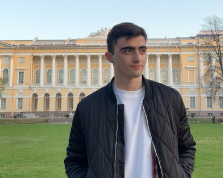
\includegraphics[width=\textwidth]{tinder-photo/khakim.png}

\xbox[green]{MLE} \xbox{LR} \xbox[blue]{CLT}

\begin{mybox}
Для любых случайных величин $X,Y$ верно: 
\[
\Var(X) = \E[\Var(X | Y)] + \Var(\E[X | Y]).
\]
\end{mybox}
\end{tinderm}
\end{minipage}

\begin{minipage}{0.45\textwidth}
\begin{tinderm}{Askhab 20}
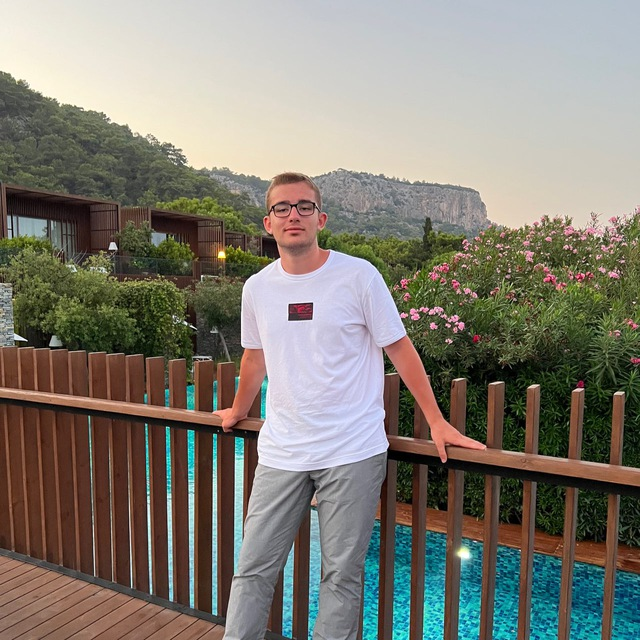
\includegraphics[width=\textwidth]{tinder-photo/askhab.jpg}

\xbox[green]{GMM} \xbox{Bayes} \xbox[blue]{LLN}

\begin{mybox}
Для биномиального распределения верно: 
\[
\sum_{k=0}^{n} C_{n}^{k} p^{k} (1-p)^{n-k} = 1.
\]
\end{mybox}
\end{tinderm}
\end{minipage}
%
%
\begin{minipage}{0.45\textwidth}
\begin{tinderf}{Alina 19}

\includegraphics[width=\textwidth]{tinder-photo/alina.jpg}

\xbox[green]{CLT} \xbox{Jensen's Inequality} \xbox[blue]{LLN}

\begin{mybox}
Корректная формула Байеса для событий $B, A_{1,N}$: 
\[
\P(A_{j}\mid B) = \frac{\P(B \mid A_{j})\P(A_{j})}{\sum_{i=1}^{N} \P(B \mid A_{i})\P(A_{i})}.
\]
\end{mybox}
\end{tinderf}
\end{minipage}
\newpage
%
\begin{minipage}{0.45\textwidth}
\begin{tinderm}{Ivan 21}

\includegraphics[width=\textwidth]{tinder-photo/ivan.jpg}

\xbox[green]{OLS} \xbox{ONS} \xbox[blue]{GARCH}

\begin{mybox}
Если $\xi_1, \dots, \xi_n$ н.о.р.с.в, $n \ge 2$ и $\eta_i = \xi_i /(\xi_1 + \dots + \xi_n)$, то 
\[
\Cov(\eta_i, \eta_j) < 0\text{ при } i \neq j.
\]
\end{mybox}
\end{tinderm}
\end{minipage}
%
%
\begin{minipage}{0.45\textwidth}
\begin{tinderm}{Maxim 20}
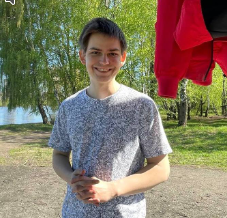
\includegraphics[width=\textwidth]{tinder-photo/maxim.png}

\xbox[green]{Poplar} \xbox{Trees} \xbox[blue]{Random forest}

\begin{mybox}
Для любых случайных величин $X,Y$ верно: 
\[
\E[\E[X | Y]] = \E[X].
\]
\end{mybox}
\end{tinderm}
\end{minipage}

\begin{minipage}{0.45\textwidth}
\begin{tinderm}{Artem 20}

\includegraphics[height=7cm]{tinder-photo/artem.png}

\xbox[green]{Stochan} \xbox{LATE} \xbox[blue]{Wiener process}

\begin{mybox}
Для любой случайной величины $X$ верно:  
\[
\E(X | X > 0) \ge \E(X).
\]
\end{mybox}
\end{tinderm}
\end{minipage}
%
%
\begin{minipage}{0.45\textwidth}
\begin{tinderm}{Timur 20}

\includegraphics[height=7cm]{tinder-photo/timur_2.png}

\xbox[green]{Bootstrap} \xbox{GitHub} \xbox[blue]{ML}

\begin{mybox}
Если $\P(B)=1$, то 
\[
\P(A|B) + \P(A|B^c) = 1.
\]
\end{mybox}
\end{tinderm}
\end{minipage}

\newpage

%
\begin{minipage}{0.45\textwidth}
\begin{tinderf}{Polina 29}

\includegraphics[width=\textwidth]{tinder-photo/polina.jpg}

\xbox[green]{BTC} \xbox{GARCH} \xbox[blue]{GLS}

\begin{mybox}
Если события  $A$ и $B$ независимы, то события $A^c$ и $B^c$ тоже независимы.
\end{mybox}
\end{tinderf}
\end{minipage}
%
\begin{minipage}{0.45\textwidth}
\begin{tinderf}{Polina 29}

\includegraphics[width=\textwidth]{tinder-photo/polina.jpg}

\xbox[green]{BTC} \xbox{GARCH} \xbox[blue]{GLS}

\begin{mybox}
Если события  $A$ и $B$ независимы, то события $A^c$ и $B^c$ тоже независимы.
\end{mybox}
\end{tinderf}
\end{minipage}
%



\begin{minipage}{0.45\textwidth}
\begin{tinderf}{Polina 29}

\includegraphics[width=\textwidth]{tinder-photo/polina.jpg}

\xbox[green]{BTC} \xbox{GARCH} \xbox[blue]{GLS}

\begin{mybox}
Если события  $A$ и $B$ независимы, то события $A^c$ и $B^c$ тоже независимы.
\end{mybox}
\end{tinderf}
\end{minipage}
%
\begin{minipage}{0.45\textwidth}
\begin{tinderf}{Polina 29}

\includegraphics[width=\textwidth]{tinder-photo/polina.jpg}

\xbox[green]{BTC} \xbox{GARCH} \xbox[blue]{GLS}

\begin{mybox}
Если события  $A$ и $B$ независимы, то события $A^c$ и $B^c$ тоже независимы.
\end{mybox}
\end{tinderf}
\end{minipage}


\newpage


\section{Задача на разрезание и письмо}

\vspace*{1cm}

\begin{huge}
Машка гадает на волшебной ромашке про Ромку.
С Ромкой возможно одно из четырёх \\
равновероятных событий: любит, не любит, к чёрту пошлёт, к сердцу прижмёт. 
Волшебная ромашка знает отношение Ромки к Машке.
При гадании ромашка подскажет Машке верный ответ \\ 
с вероятностью 0.4, а каждый из трёх неверных — с вероятностью по 0.2. 

Какова условная вероятность события «к сердцу прижмёт»,
если ромашка подсказывает, что Ромка любит Машку?
\end{huge}

% решение 
% 
%
%\[
%\P(A \mid B) = \frac{0.25 \cdot 0.2}{0.25 \cdot 0.4 + 0.75 \cdot 0.2} = %0.2
%\]



\vspace*{2cm}

    Клайд получил от Бонни валентинку:

\vspace*{1cm}
 
Мой милый Клайд, каждый день я шлю тебе случайное пуассоновское количество сообщений с ожиданием 100 штук.  
Каждое сообщение я равновероятно отправляю либо своими дрожащими на\-ма\-ни\-кюренными пальчиками, либо своим дрожащим голосом. 
Если я отправляю более 70 сообщений пальчиками, 
то мне нужно восстановить маникюр, на что я трачу равномерное время от одного часа до двух часов. Почему ты мне вчера ни разу не написал?
Моим страданиям нет меры и ещё равномерное время от двух часов до трёх часов я провожу у своего личного психоаналитика. 

    
%    Меня зовут Наталья. Я преданная читательница вашего журнала уже 20 лет. 
%    Расскажу немного о себе. Каждый день я варю борщ. Время приготовления борща имеет экспоненциальное распределение. До замужества я тратила на один борщ в среднем 30 минут.
%    У меня в натальной карте 5 указаний на развод. 
%    Каждое указание на развод повышает ожидаемое время приготовления борща на $10$ минут. 
%    Я живу 10 лет с мужем и у нас все хорошо. Мы разведемся?

\vspace*{1cm}

Помогите Клайду ответить на валентинку. 





\end{document} 